\documentclass[oneside]{book}
\usepackage[utf8]{inputenc}
\usepackage{graphicx}
\usepackage{placeins}
\usepackage{amsmath}
\usepackage{geometry}
\usepackage{listings}
\lstset{
breaklines=true,
postbreak=\mbox{\textcolor{red}{$\hookrightarrow$}\space},
numbers=left, 
numberstyle=\small, 
numbersep=8pt, 
frame = single, 
framexleftmargin=15pt}
\usepackage[backend=biber,style=alphabetic,sorting=ynt]{biblatex} 
\usepackage{hyperref}
\hypersetup{
    colorlinks=true,
    linkcolor=blue,
    filecolor=magenta,      
    urlcolor=cyan,
    pdftitle={Overleaf Example},
    breaklinks=True,
    pdfpagemode=FullScreen,
    }

\urlstyle{same}
\addbibresource{Validation_template_user_manual.bib}
\title{RAVEN Template documentation}
\author{Marisol Garrouste}
\date{February 2022}

\begin{document}

\maketitle

\newpage
\chapter{User documentation}
\section{Input file description}


%The user's documentation has not been developed as much as it should be for practical use. One of the next goals for this template  - however outside the scope of this project - is indeed to change the format of the user input file to \verb|XML|. This new format will enable better integration of the Validation template within the RAVEN framework since all RAVEN's and RAVEN plugins' inputs should be written as \verb|XML| files. Furthermore an \verb|XML| format will permit the (re-)use of RAVEN input data classes and thus allow for better testing coverage as well as automatic documentation generation. 

%The existing documentation can be found in the following project folder : \\\verb|\RAVEN-Validation-Template\doc\|; and several examples, based on the Dymola Pendulum model, detailed in the following sections are also available ( \verb|\RAVEN-Validation-Template\tests\| ).


The input file is setup as a configuration file: options organized in sections should be provided by the user as in File \ref{input:config_file} . 
The various sections and options will be described in the following paragraphs. 
\begin{lstlisting}[language=make,caption={Configuration file format}, label={input:config_file}]
[SECTION]
option1 = option1_value  
option2 = option2_value
\end{lstlisting}

\FloatBarrier

\subsection{CASE}

\subsubsection{type} Required : type of analysis to perform
\\Allowed values: 
\begin{itemize}
    \item \verb|calibration|
    \item \verb|validation|
\end{itemize}

\subsubsection{metric} Required : metric used to compute the difference between the model and the experimental data
\\Allowed values: 
\begin{itemize}
    \item \verb|mean_absolute_error|
    \item \verb|DTW|
    \item \verb|mean_squared_error|
    \item \verb|euclidean|
\end{itemize}


\subsection{MODEL}

\subsubsection{dymola\_exe} Required: path to the executable file for the Dymola model of interest

\subsubsection{dymola\_ini} Required: path to the initialization file for the Dymola model of interest

\subsubsection{targets} Required: quantity of interest in the model
\\First value: Alias for the target in the RAVEN script
\\Second value: Path of the target in the Dymola model

\subsection{ROM}

This section is optional, if it is written a ROM RAVEN training input file will be generated and the calibration RAVEN script will point to the reduced order model instead of the initial Dymola model.  

\subsubsection{type} Required: type of reduced order model to train
\\Allowed values:
\begin{itemize}
    \item \verb|DMD|
    \item \verb|PolyExponential|
    \item \verb|SyntheticHistory|
\end{itemize}

\subsubsection{sampler} Required: type of sampling used to generate the training points for the reduced order model
\\Allowed values: 
\begin{itemize}
    \item \verb|Stratified|
    \item \verb|MonteCarlo|
\end{itemize}

\subsubsection{grid\_size} Required: number of training points for the reduced order model
\\Allowed values: integer

For each kind of reduced order model different options should be provided by the user. They are specified in the following paragraphs. The user should refer to the RAVEN user \cite{rabiti_raven_2021} and theory \cite{alfonsi_raven_2021} manuals to understand how to use each option. 

\subsubsection{DMD}
\begin{itemize}
    \item \verb|dmdType|
    \item \verb|rankSVD|
    \item \verb|optimized|
    \item \verb|exactModes|
    \item \verb|rankTLSQ|
    \item \verb|energyRankSVD|
\end{itemize}


\subsubsection{PolyExponential}
\begin{itemize}
    \item \verb|numberExpTerms|
    \item \verb|tol|
    \item \verb|max_iter|
    \item \verb|coeffRegressor|
\end{itemize}

\subsubsection{SyntheticHistory}
\begin{itemize}
    \item \verb|fourier|
    \item \verb|wavelet|
\end{itemize}

\FloatBarrier
\subsection{EXPERIMENT}
\subsubsection{dataset} Required: path to the experimental dataset file (csv)
\\Note on the file format: For RAVEN to load the data the file should include the values of the parameters (see Figure \ref{fig:dummy_exp_values}) and the address of a second csv file with the corresponding target time series (see Figure \ref{fig:values}). 

\begin{figure}
    \centering
    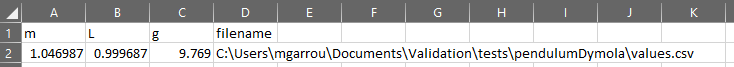
\includegraphics[width=\textwidth]{pics/dummy_exp_values.PNG}
    \caption{Main csv file with parameters values and path to time series data file}
    \label{fig:dummy_exp_values}
\end{figure}

\begin{figure}
    \centering
    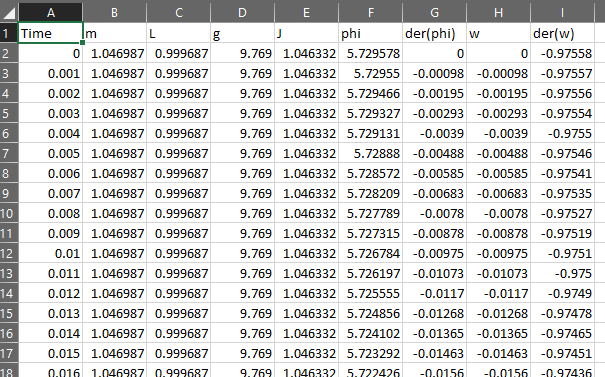
\includegraphics[width=\textwidth]{pics/values.PNG}
    \caption{Time series data file}
    \label{fig:values}
\end{figure}


\subsubsection{targets} Required: name of the target variable in the experimental dataset

\subsubsection{post\_process} Required: Whether a post-processing script should be run to format the experimental data before trying to load it into RAVEN
\\Allowed values: Boolean

\subsubsection{post\_process\_script} Required if post\_process: path to the experimental data post-processing script

\FloatBarrier

\subsection{VARIABLES}
For each parameter the following information should be provided by the user

\subsubsection{\$name\_of\_variable}
Required: 
\begin{enumerate}
    \item Name of parameter in Dymola model
    \item Name of parameter's distribution
    \\Allowed values: 
    \begin{itemize}
        \item \verb|Uniform|
        \item \verb|Normal|
    \end{itemize}
    \item Numerical parameters defining the parameter's distribution
    \\For instance \$mean, \$standard\_deviation for a normal distribution
\end{enumerate}


\subsection{OPTIMIZATION}
This section is required when the user indicated that a calibration is being performed in the \verb|[CASE]| section. 

\subsubsection{max\_iterations}
Required: Maximum number of iterations for the calibration optimization. 
\\Allowed values: integer

\subsubsection{nb\_traj}
Required: Number of optimization trajectories (i.e. restarts)
\\Allowed values: integer

\subsubsection{\$variable}
Required: List of starting values for the optimization parameters, the number of starting values must be the same of the number of trajectories
\\Allowed values: list of floats

\subsection{SETTINGS}
This section is optional, the user can provide folders' and files' names for the RAVEN scripts being generated. Use of this section is recommended to avoid over-writing previously generated files. 

\subsubsection{work\_dir}
Optional: Name of the RAVEN working directory

\subsubsection{calibration\_file}
Optional: Name of the RAVEN calibration file

\subsubsection{validation\_file}
Optional: Name of the RAVEN validation file

\FloatBarrier
\section{Pendulum example}

\subsection{Calibration with ROM}

The input presented below (File \ref{input:pendulum_cal_rom}) is an example of an input for the RAVEN Validation template that will lead to the generation of RAVEN XML input files to perform the calibration of the Pendulum model via a ROM. 3 files will be generated, the Figure \ref{fig:sequence_calibration_w_ROM} shows the main steps performed by RAVEN when these files are run successfully:
\begin{itemize}
    \item a ROM training script, running this file with RAVEN will create a ROM and train it on data from the Pendulum Dymola model and then saved it to a file for latter use. 
    \item a calibration XML file: running this file with RAVEN will perform an optimization of the Pendulum Dymola model's parameters with the distance between the ROM data and the experimental data as a target
    \item a validation XML file: this file is linked to the calibration file and runs a second instance of RAVEN that will compute the distance between the ROM data and the experimental data and pass these values to the calibration script. 
\end{itemize}
\begin{figure}
    \centering
    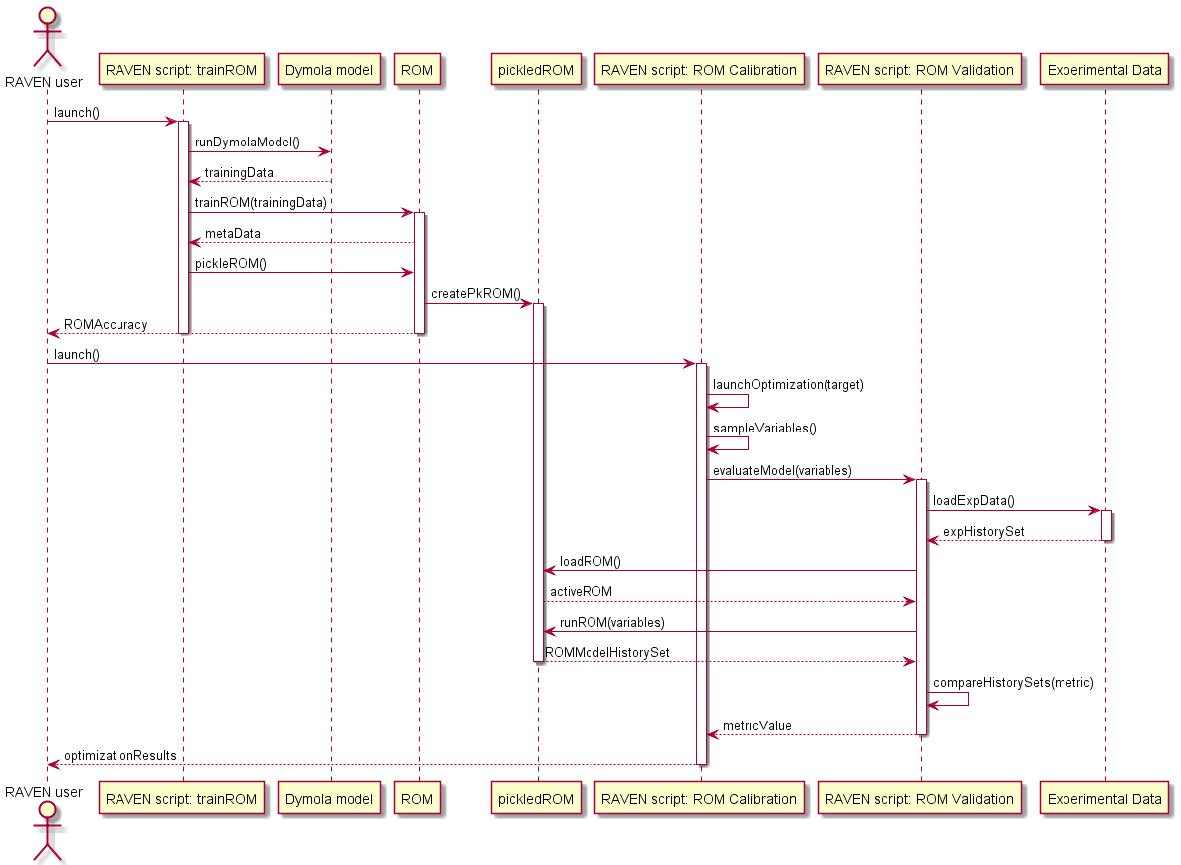
\includegraphics[width=0.99\textwidth]{pics/sequence_calibration_w_ROM.jpg}
    \caption{Sequence diagram: RAVEN calibration with ROM}
    \label{fig:sequence_calibration_w_ROM}
\end{figure}
\FloatBarrier

\begin{lstlisting}[language=make,caption={Pendulum input file, Calibration with ROM}, label={input:pendulum_cal_rom}]
[CASE]
type = calibration  
metric = mean_absolute_error

[MODEL]
dymola_exe= C:\Users\mgarrou\Documents\Validation\tests\pendulumDymola\dymosim.exe
dymola_ini = C:\Users\mgarrou\Documents\Validation\tests\pendulumDymola\dsin.txt
targets = Angle, phi

[ROM]
type = DMD
dmdType = dmd 
rankSVD = 0
optimized = True 
exactModes = True
sampler = Stratified
grid_size = 50

[EXPERIMENT]
dataset = C:\Users\mgarrou\Documents\Validation\tests\pendulumDymola\dummy_exp_values.csv
targets = phi
post_process = False

[VARIABLES]
mass = m, Uniform, 0.1, 10
length = L, Uniform, 0.1, 2.0
gravity = g, Uniform, 9.0, 11.0

[OPTIMIZATION]
max_iterations = 100
nb_traj = 3
mass = 0.2,5,7
length = 0.2,0.5,0.7
gravity = 9.5, 10.0, 10.5

[SETTINGS]
work_dir = pendulum_cal_rom
calibration_file = pendulumCalibration
validation_file = pendulumValidation
\end{lstlisting}



The file presented in \ref{input:pendulum_cal} shows an example of a calibration. The process is similar to the one exposed in the previous paragraph; the difference lies in the fact that no ROM of the Dymola model is used. Thus the target of the optimization is now the distance between the experimental data and the Dymola model data. 

\FloatBarrier
\subsection{Calibration}

\begin{lstlisting}[language=make,caption={Pendulum input file, Calibration}, label={input:pendulum_cal}]
[CASE]
type = calibration  
metric = mean_absolute_error

[MODEL]
dymola_exe= C:\Users\mgarrou\Documents\Validation\tests\pendulumDymola\dymosim.exe
dymola_ini = C:\Users\mgarrou\Documents\Validation\tests\pendulumDymola\dsin.txt
targets = Angle, phi, Angular_velocity, w

[EXPERIMENT]
dataset = C:\Users\mgarrou\Documents\Validation\tests\pendulumDymola\dummy_exp_values
targets = phi, w
post_process = False

[VARIABLES]
mass = m, Uniform, 150, 0.1, 10
length = L, Uniform, 100, 0.1, 2.0
gravity = g, Uniform, 50, 9.0, 11.0

[OPTIMIZATION]
max_iterations = 100
nb_traj = 3
mass = 0.2,5,7
length = 0.2,0.5,0.7
gravity = 9.5, 10.0, 10.5

[SETTINGS]
work_dir = pendulum_cal
calibration_file = pendulumCalibration
validation_file = pendulumValidation
\end{lstlisting}


\FloatBarrier
\subsection{Validation}

Finally the input file \ref{input:pendulum_val} shows a validation example, the Pendulum Dymola model results are compared to the experimental data and the resulting distance value provided an accuracy estimate of the model to the user. 

\begin{lstlisting}[language=make,caption={Pendulum input file, Validation}, label={input:pendulum_val}]
[CASE]
type = validation
metric = mean_absolute_error

[MODEL]
dymola_exe= C:\Users\mgarrou\Documents\Validation\tests\pendulumDymola\dymosim.exe
dymola_ini = C:\Users\mgarrou\Documents\Validation\tests\pendulumDymola\dsin.txt
targets = Angle, phi, Angular_velocity, w

[EXPERIMENT]
dataset = C:\Users\mgarrou\Documents\Validation\tests\pendulumDymola\dummy_exp_values.csv
targets = phi, w
post_process = False

[VARIABLES]
mass = m, Uniform, 150, 0.1, 10
length = L, Uniform, 100, 0.1, 2.0
gravity = g, Uniform, 50, 9.0, 11.0

[SETTINGS]
work_dir = pendulum_val
validation_file = pendulumValidation
\end{lstlisting}

















\FloatBarrier
\chapter{Developer documentation}

The RAVEN Validation Template is for now useful only to calibrate or validate Dymola models. However RAVEN can be coupled to various other codes such as those included in the MOOSE framework. This template could thus be extended to include the ability for users to generate calibration and validation file for models written for these simulations codes. 

The developer documentation is thus an important step to make sure this template can be further developed and its capabilities extended. To this end, docstrings and inline comments have been written to inform about the purpose of each method as well as precise the logic behind the structure of the code if not obviously clear. 

The code in \ref{python:ValidationTemplate} is an example of this documentation. This purpose of the class is described at first. The constructor for this class takes in dictionary of options supported by the template for the metric and the distributions. The next method shown is \verb|createWorkflow|, this method is the main one called to fill out the incomplete XML file. It therefore needs to take in a lot of information about the validation process as a whole: the model, the experimental data, the variables,... All the information is stored in dictionaries with consistent keys across all files and objects of the RAVEN Validation Template. 

\begin{lstlisting}[language=Python, caption={Validation Template Class}, label={python:ValidationTemplate}]
class ValidationTemplate(Template):
    """
    Template class to create the validation file for the RAVEN validation template
    """

    def __init__(self, metrics, distributions, calibration):
        """ 
        Validation Template Constructor 
            @ In, metrics, dict, dictionary of metrics implemented with information
            @ In, distributions, dict, dictionary of distributions implemented with information
            @ In, calibration, boolean, indicates if the validation XML file will be used for calibration
            @ Out, None 
        """
        super(ValidationTemplate, self).__init__()
        self.metrics = metrics
        self.distributions = distributions
        self.calibration = calibration
    
    # =============================================================================
    #     API methods
    # =============================================================================
    
    def createWorkflow(self, model=None, exp=None, variables=None, metric=None, romTag=False, **kwargs):
        """
        Creates a new RAVEN workflow file based on the information in kwargs.
        Specific to individual templates. Must overload to be useful.
            @ In, romTag, bool, whether validation workflow should be written for 
            @ In, model, dict, information about the model
            @ In, variables, dict, information about the variables, dictionary of dictionary 
                each variable dictionary has with the following keys : 
                    - path, str: path of the variable in the model 
                    - distribution, str: probability distribution name 
                    - dist_params, list[float]: numerical parameters defining the PDF
                    - alias, str: alias of the variable in the RAVEN XML file
            @ In, metric, str, metric used to compute the distance bet. model and exp data 
            @ In, romTag, bool, indicates whether or not a ROM is used for calibration
            @ In, kwargs, dict, other unused keyword arguments
            @ Out, xml.etree.ElementTree.Element, modified copy of template
        """
        template = Template.createWorkflow(self, **kwargs)
        # Fill variables list
        allVars = list(variables.keys())
        # Adjust Files block: Dymola initialization and experimental data
        if romTag: 
            self._addFile(xml=template, fileName='romPk', path='trainROMWorkDir\\romPk', ftype='')
            inputNode = template.find("Steps").find("IOStep[@name='loadROM']").find('Input')
            self._updateCommaSeperatedList(inputNode, "romPk")
        else:
            self._addFile(xml=template, fileName='dsin.txt', path= model['dymola_ini'], ftype='DymolaInitialisation')
        if exp['pp']:
            self._addFile(xml=template, fileName='expInput', path=exp['clean_dataset'])
        else:
            self._addFile(xml=template, fileName='expInput', path=exp['dataset'])
        # Add variables
        for var in allVars:
            if self.calibration: 
                self._addInputVariableForCalibration(xml=template, varPath=variables[var]['path'], romTag=romTag)
            else:
                self._addInputVariableForValidation(xml=template, varName=var, varDict=variables[var])
        # Metric 
        # Syncing post processor if basic metrics used
        self._addMetric(xml=template, metric=metric)
        if metric != 'DTW':
            self._addSync(template, metric=metric)
        for targetCodeAlias, targetExpName in zip(model['targets'].keys(), exp['targets']): 
            path = model['targets'][targetCodeAlias]
            self._addTarget(xml=template, targetExpName=targetExpName, 
                targetCodeAlias=targetCodeAlias, targetCodePath=path, metric=metric, romTag=romTag)
        # Add executable to Code
        if not romTag:
            template.find('Models').find('Code').find('executable').text = model['dymola_exe']
        return template
\end{lstlisting}

\medskip
\printbibliography




\end{document}
